\chapter{Approach}
\label{chapter:approach}


% [Last chapter]

% [This chapter: Describe shortly all sections from this chapter]

%- In this chapter the practical work should be documented and explained
%- Elaboration of how the practical work could help answer the research question
%- Discussion of real-life setup and how experiments approach it


% [In the next chapter]

%- Evaluation of data is in next chapter


% ------------------------------------------------------------------------------------------

\section{Introduction to Empirical Research Methods}


% Overview of methods

% reproduceability, validity etc

% Justification why following approaches are conducted as controlled experiments


% 2005 Sjoberg: experiments in computer science evaluation

% 2006 Wohlin
% Quantitative: Experiment, Case study, Survey, post-mortem analysis

% 2008_Mytkowicz Observer effect

% 2012 Maxion: Hallmarks of good experiment, Validity

% 2014 Tedre: Experimentation in computing


% 2016 Kohavi p. 4, p.5 planning an experiment


% --------------------------------------------------------


\subsection{Controlled Experiments in Computer Science}


% Short overview about controlled experiments in computer science
% Design: Show test setup image: Independent and dependent variables
% Hypothesis testing


% 2006 Wohlin:
% Design, analysis and interpretation

% 2014 Tedre: Controlled experiments

% Measuring Real User Performance in the Browser: Avoiding the Observer Effect



% ------------------------------------------------------------------------------------------


\section{Experiment / Test Setup / Design}

% [Research Question]

The research question is... as explained in section X.
One way to approximate answers is with the following experiment.


% [Design]

The goal of the experiment is to measure / observe changes if the tracking script, instrumented by the independent variables, changes the performance of the website, instrumented by the dependent variables.

The setup consists of five parts (figure X):

a) Independent Variables Specific changes in test object (see next chapter)

b) Dependent Variables; Performance metrics

c) Test Object: Website, see section X.

d) RUM

e) Synthetic Monitoring

The different parts will be discussed in more detail below.

\begin{figure}[h!]
\begin{center}
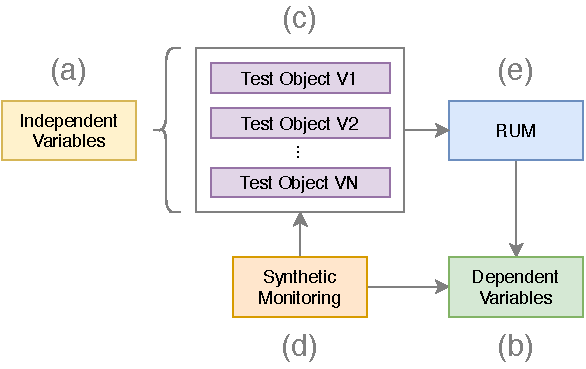
\includegraphics[width=0.8\textwidth]{design.pdf}
\caption{Components from the Controlled Experiment}
\label{figure:design_setup}
\end{center}
\end{figure}



% Kohavi 2016: Sample size, collect right metrics, track right users, randomization unit


% --------------------------------------------------

\subsection{Independent Variables}

% [What are they representing]

As will be explained in section X, the test object is a website, a main HTML document to be precise.
I want to see if and how the tracking script influences the performance of the website.
The independent variables reflect how the tracking script is included into the website.

% [Page Tagging]

As described in section X, page tagging is the method of choice of including a tracking script into a website.
Different configurations and options exist of how to include a script into a website.
The independent variables reflect those options (table X).

\begin{table}[h]
	\small
	\centering
	\begin{tabular}{ | l | l | }
	\hline
	Independent Variable \cellcolor{lightgrey} & Possible Values \cellcolor{lightgrey} \\
	\hline
	Position of the Tracking Script & top-head, bottom-head, bottom-body \\
	Attribute of the Tracking Script & none, async, defer \\
	Other Tracking Script included & no, yes \\
	\hline
	\end{tabular}
	\medskip
	\caption{Independent Variables}
	\label{table:independent_variables}
\end{table}

% [Comparison]

When evaluating,I will compare the values from one independent variable only.
Therefore, when comparing the values of one independent variable, i need to set a default value for the other independent variables.

Each IV is explained in more detail below.

Of course theoretically there are unlimited possible IVs.
Some examples are described in section X.

% -------------------------

\subsubsection{IV 1: Position of the Tracking Script}

I use GA.

Multiple options exist.

What is Google suggesting?

% [GA Tracking Code]

% Grigorik Conference Talk https://www.youtube.com/watch?v=PkOBnYxqj3k&ab_channel=IlyaGrigorik
% And slides https://www.igvita.com/slides/2013/fluent-perfcourse.pdf


% https://developers.google.com/analytics/devguides/collection/analyticsjs
%- this async pattern is used so that all browsers will load it async
%- we can just use async attribute for newer browsers...


% [Explanation]

What is the GA script doing?
Actually, it creates another async script tag which loads the actual analytics JS.
So basically it should not really play a role where we place it.
Evaluation will show.

What does the code snippet do?
Basically the sync part is only..
It creates another script tag which is async and which loads the tracking code.


% [Other examples]

Other vendors suggest other positions.

% From Hotjar installation page: "Paste the Hotjar code into the <head> of every page you wish to track users and collect feedback. And then verify your installation."

% Show multiple code examples
% Explain whats going on: script tag, create script element etc.
% Maybe also show Hotjar example to see that they are similar


% Compare how GA script is included into web site with some other analytics services examples
% Some other real life examples of RUM here? To demonstrate async... boomeraing readme for example has nice explanation


% https://speedcurve.com/setup/lux/
% SpeedCurve tracking script position: To add real user monitoring (RUM) to your site, paste this snippet at the top of the <HEAD> tag on your pages.

% see appendix X

% -------------------------

\subsubsection{IV 2}

As explained above, inside the GA tracking code snippet, another script tag with the attribute async is created.
Async has the effect, that..., as explained in section X.

As described in section X. async and defer attributes on inline scripts are ignored, see section X.
"Inline JavaScript script tags ignore the defer or async attribute"
As the "wrapper" snippet is a inline script (no src attribute), the attributes on this script tag should not have any effect.
Still, as many suggest to add them, i will test this as well.

I expect that changing this variable has no impact.
Evaluation shows that...

% for a code example of IV 2, see appendix X


% -------------------------

\subsubsection{IV 3}

Many websites use multiple RUM / tracking scripts.
%show some examples

Do they effect each other?

From technical perspective, loading another script will take some extra time, depending on network, connection, bytes needed to transfer etc.

With changing this IV, we can see the impact of it in evaluation.


% see appendix X

% -------------------------

\subsubsection{Other IVs not included but worth mentioning}

% More or less infinite number of independent variables
% Again the big and important fact that each website is different


% -------------------------

\subsubsection{Possible Variations of the Independent Variables}

When combining all IVs, different variations occur (table X).

% as described before, i will compare the values within one independent variable. 
% This is needed in order to compare the impact of the different values within one IV.
% For example, i want to measure if there is a difference in performance between the different script attributes. To measure this, i set the default values for the other IVs and vary the values for the IV attribute


\begin{table}[h]
	\small
	\centering
	\begin{tabular}{  | c || c | c | c | } 
	\hline
	Variant & Position & Attribute & Other Scripts \\
	\hline \hline
	Variant P1 & top-head & \cellcolor{lightgrey} none & \cellcolor{lightgrey} no \\
	   Variant P2 & bottom-head & \cellcolor{lightgrey} none & \cellcolor{lightgrey} no \\
	   Variant P3 & bottom-body & \cellcolor{lightgrey} none & \cellcolor{lightgrey} no \\
	  \hline
	   \sout{Variant A1} & \cellcolor{lightgrey} \sout{top-head} & \sout{none} & \cellcolor{lightgrey} \sout{no} \\
	   Variant A2 & \cellcolor{lightgrey} top-head & async & \cellcolor{lightgrey} no \\
	   Variant A3 & \cellcolor{lightgrey} top-head & defer & \cellcolor{lightgrey} no \\
	  \hline
	  \sout{Variant OS1} & \cellcolor{lightgrey} \sout{top-head} & \cellcolor{lightgrey} \sout{none} & \sout{no} \\
	  Variant OS2 & \cellcolor{lightgrey} top-head & \cellcolor{lightgrey} none & yes \\
	  \hline
	\end{tabular}
	\medskip
	\caption{Test Object Variants}
	\label{table:test_object_variants}
\end{table}

% [Table Explanation]

Some variants are there twice:
Hence i will cut out variants X and Y.


% [Comparison]

% I will not compare variants which are not from the same subgroup, e.g. Variant A2 will not be compared to Variant OS2.
% Because the first row of the variants table also includes the default values for Attribute and Other Scripts, VP1 is equal to VA1 and VO1.

% With the defined IVs and variants, I can create the test objects, that is the index.html files with the corresponding setup.
% Because its easier to differentiate i will create for the three equal variants nevertheless own index files.

% For each test variant, I will create a concrete test artefact, which is a modified index.html.
% This index.html needs to be uploaded to the webserver before starting with the tests.

% All variants will have the same name which is index.html. This is the default file which will be delivered by the webserver when accessing root path of webpage.



% --------------------------------------------------


\subsection{Dependent Variables}

% Measure effects
% Performance metrics from Lab and Field, see terms and definitions
% But also quality of RUM data. Because we could have a nice performance but RUM will be of bad quality

\subsubsection{Page Weight}

	- Bytes
	- Requests

\subsubsection{Measures from Synthetic Monitoring}

Categories explained in section X.
WPT measures this in section X.

I will measure this:

- Navigation Timing Metrics:
	- TTFB
	- Document Complete
	- Fully Loaded
	
- User-Centric Metrics:
	- FCP
	- Speed Index
	- LCP
	- CLS

\subsubsection{Measures from RUM}

GA tracks this, as explained in section X.

- PLT
- Page Download Time
- Server Connection Time
- Domain Lookup Time
- Redirection Time
- Server Response Time
- Domain interactive time
- Domain Content Loaed Time



% --------------------------------------------------

\subsection{The Test Object: An E-Commerce Website}

% Ideal: Use a real website. Is not possible
% Mimic the website is one thing, but also all other aspects should be fairly similar: infrastructure (hosting), hardware used, network speed, traffic, etc.
% This experiment/test is only an approximation and can serve as a starting point for further investigations

% Concrete File to mimic: HTML Template / document with all other resources that build up the website: CSS, JS, Fonts, Images, Videos, etc.

% Depending on different approaches / Ideas (see next chapter), template looks different
% But general structure stays the same and independent variables can be defined
% Here we show different independent variables and variants

% Several ideas are proposed
% Each idea has pro and contra: each idea should be discussed of its usefulness, advantages and disadvantages

% skeletal explained in section X, wordpress in section X, etc.


% --------------------------------------------------------

\subsubsection{Plain / Skeletal Website}


% [Why]
% Idea: Lab environment to have control over all and see effects of changing independent variables
% Use this as the simplest test possible, not even POC (POC is http archive site)
    
% [Setup]
% website: simple html document
% Hosting: github pages

% [Evaluation]
% Problem: Too far away from reality

% --------------------------------------------------------

\subsubsection{"Median" Website from HTTP Archive}


% [Why]
% Idea: Get correct page weight

% [Setup]
% website: mimic page weight as reported on http archive
% Hosting: github pages

% [Evaluation]
% Only good as a POC: Show that changing independent variables X affect result
% too far away from reality
% maybe compare with real website ?


% 2011 Butkiewicz: Correlation between website complexity and its performance:
% -> Therefore it makes sense for me to use http archive inspired website approach, since page weight / page complexity impacts performance
% - Measures impact of website complexity on performance
% - Finds out that top 5 metrics that determine performance are:
% total number of objects loaded,  the number of these objects that are Javascripts,  the total web- page size,  and the number of servers and origins contacted in loading objects on the page.


% 2011 Grigorik Anatomy of modern web application
% - Chart with changes on time: apps are growing


% 2014 Hogan basics-of-page-speed/ What Is the HTTP Archive?


% --------------------------------------------------------

\subsubsection{WordPress}


% [Why]
% Show usage of WordPress with some statistics: Why is it so verbreitet

% [Plugins]
% Explain Plugin system

% WooCommerce

% [Setup]
% Explain Setup on localhost with wocommerce and GA plugin

% [Evaluation]
% Elaborate why this idea was not used



% --------------------------------------------------------


\subsubsection{Mirroring a complete e-commerce website}


% [Why]

% Close to reality as possible


% Idea: Close to reality as possible
% Problems when mirroring a website
% Elaborate why this idea of mirroring complete website was not used
% I used mock of start page of otto, which works fine
% Compare original otto website with mock


% Why Otto and Zalando ?Which website / shop to clone? Show some statistics about biggest e-commerce websites in germany




% [Setup]

% Tool support to mirror / download complete website: httrack and chrome plugin
% Use free hosting service to serve website

% Otto first try
% Zalando final version

% [Evaluation]
% see evaluation chapter


% --------------

\paragraph{Otto}


% [Manual Adjustments]

% Manual adjustments needed:
% - Move everything to test folder because top domain is /otto


% What did not work (mostly 404s):
% - user-set-consent-id-cookie: Cookie with name consentId is not set, user-set-consent-id-cookie returns therefore 404
% - subscribeToNewsletterSnippetContent: Change path did not work...
% - amount.json: Not found, also wl\_miniWishlistAmount in local storage does not created
% - a\_info: Mock a\_info response json does not work...

% - footer
% - userTiming


% WPT RV is returning empty csv when 404s are encountered.
% Therefore i mock the missing ressources so that WPT can run bulk tests successfully.

% - mock image sprite\_all\_1ba408b2.png

% - create empty file called user-set-consent-id-cookie

% - change path for subscribeToNewsletterSnippetContent: This will remove the cookie banner... but then WPT works



% -------------------

\subparagraph{Comparison to original webpage}

% Maybe use here just WPTs comparison tool

% Show some diagrams here
% The other diagrams with Zalando should go into evaluation chapter



% -----------

\subparagraph{Problem with Caching and Repeat View}

% - Problem with RV, Caching:
% Otto sets request headers to cache-control: no-cache which means that RV basically downloads all resources again.
% The mock is hosted on Github, where the cache-control header is set to ...
% It is not possible to change the github request headers. We can modify the http request headers via html, but this is not a clean solution.
% Therefore I use a different e-commerce website which does not shut down caching so that the RV results are more similar.

% Ideally I would host the mock website on a similar infrastructure as the original site with the same webserver configuration. This is for a masters thesis not feasible.

% Not possible to set cache control in html meta tag https://html.spec.whatwg.org/multipage/semantics.html#attr-meta-http-equiv


% --------------------------------------------------------

\paragraph{Zalando}

% [Why]

% Idea: It looks like zalando page does not has that many cache-control headers, therefore it may be easier to clone so that RVs are more similar.

% [Setup]

% use plugin to download page
% host it on github pages

% [Evaluation]

% see evaluation chapter



% --------------------------------------------------


\subsection{Synthetic Monitoring: Create Traffic and Collect Data}

% Synthetic monitoring: Double role: creats traffic which is captured by RUM, and also measured the website

% I want to collect Lab and field data for dependent variables for comparison
% This setup is a special case because lab bots (e.g. WPT) simulate at the same time real users for RUM data


% -------------------------------------

\subsubsection{WebPageTest}

% [Setup]

% Possibilites:
% use public version
% API

% Private:
%- preconfigured Amazon Web Services (AWS) AMIs
%- localhost Docker


\paragraph{Configuration}

% already described in section X.

% [FV vs RV]

% First View: "First View refers to the cold cache setup in which nothing is served locally"
%Repeat View: "Repeat View refers to the warm cache containing everything instantiated by the first view" (2016 Using WPT p. 62)


\begin{table}[h]
	\small
	\centering
	\begin{tabular}{  | c | c | } 
	\hline
	\cellcolor{lightgrey} Configuration Setting & \cellcolor{lightgrey} Option \\
	\hline
%	Test Location & Test Location \\ 
	Browser & Chrome \\
	\hline
	Connection & LAN (connection speed is determined by hotspot) \\
	Desktop Browser Dimensions & default (1366x768) \\
	Number of Tests to Run & 1 \\
	Repeat View & First View and Repeat View \\
	Capture Video & True \\
	Keep Test Private & False \\
	Label & none \\
	\hline	  
	Advanced Tab & Nothing selected \\
	Chromium Tab & Capture Dev Tools Timeline selected  \\
	Auth, Script, Block, SPOF, Custom Tabs & Nothing  \\
	Bulk Testing Tab & URL of the test website $x$ times according to test plan \\
	\hline
	\end{tabular}
	\medskip
	\caption{WPT Configuration}
	\label{table:wpt_configuration}
\end{table}




% ----------------------


\paragraph{Traffic Shaping}

% [Why]

% Network Condition is very important for performance
% Already described in section X issue with Latency vs Bandwidth

% Overview table with different settings:
% https://developer.mozilla.org/en-US/docs/Web/Performance/Understanding_latency


% Important to have stable and realistic network condition
% Chromes tool is not the best for this % see blogpost https://calendar.perfplanet.com/2016/testing-with-realistic-networking-conditions/


% [Network Link Conditioner]

% Private WPT Instance docker on mac does not allow traffic shaping functionality from WPT
% One approach: I use Network Link Conditioner from Apple to slow down the whole machine. See in same blogpost that Patrick highly recommends this
% WPT also slows down their whole machines % https://forums.webpagetest.org/t/measure-internet-speed/11593
% In general internet connection is very unstable. If i run network link conditionier with e.g. DSL each speedtest gives different results. And other test platforms such as fast.com gives also different result.
% i will use the durchschnitt in germany which seems to be 40 mbit per second. or actually i use LTE profile from network conditioner which is 50 mbit per second 


% [Hotspot]

% Solution: Use Mobile Hotspot with 50 mbit/s
% as long as internet connection is stable along all tests, it should not make a big difference because i compare the different variants. Therefore internet connection will fall out of the equation




% --------------------------------------------------


\subsection{Real-User Monitoring: Google Analytics}

% Setup: Use Unversial Analytics
% Set sample rate to 100% for speed metrics



% ------------------------------------------------------------------------------------------
% ------------------------------------------------------------------------------------------s


\section{Conducting the Experiment}


\subsection{Test Plan and Data Collection}

% The Google Analytics code is more or less fixed and there are no configurations.
% It would be possible to change config of script, e.g. change sample rate, track other metrics etc.
% But it is not possible to change default tracking behaviour (?)

% How the script is included into the file should reflected withing Website Variations

% I will use only one WPT Configuration for all tests.
% Other WPT config can be used in future work, e.g. emulate mobile device.


\begin{table}[h]
	\small
	\centering
	\begin{tabular}{ |c|c|c|c| } 
	 \hline
	  Variant \cellcolor{lightgrey} & Traffic Shaping \cellcolor{lightgrey} & Runs \cellcolor{lightgrey} & Date \cellcolor{lightgrey} \\
	  \hline
	  Original Website & 50 mbit/s & 500 & 2021-01-01 \\
	  Mock without GA included & .. & .. & .. \\
	  \hline
	  V-P1 & DSL & 500 & 2021-05-07 \\
	  V-P2 & DSL & 500 & 2021-05-07 \\
	  V-P3 & DSL & 500 & 2021-05-07 \\
	  \hline
	  V-A1 & DSL & 500 & 2021-05-07 \\
	  V-A2 & DSL & 500 & 2021-05-07 \\
	  V-A3 & DSL & 500 & 2021-05-07 \\
	  \hline
	  V-OS1 & DSL & 500 & 2021-05-07 \\
	  V-OS1 & DSL & 500 & 2021-05-07 \\
	  \hline
	  \end{tabular}
	\medskip
	\caption{Test Runs}
	\label{table:test_runs}
\end{table}


% --------------------------------------------------

\subsection{Test Protocol, Experiment Conducting Procedure}

\begin{itemize}
\item Deploy variant of index.html by pushing to GitHub
% \item Start Network Link Conditioner with specified config on local machine
\item Test internet speed with speedtest-cli
\item Start local WPT server and agent
\item Configure WPT according to specified setup and add list of urls to bulk test interface
\item Run test
\item When finished, download summary csv file
\item On GA helper site, fetch and download data for the current day
\end{itemize}



% [Transition]

% Now lets see the data in chapter X Evaluation